%%%%%%%%%%%%%%%%%%%%%%%%%%%%%%%%%%%%%%%%%%%%%%%%%%%%%%%%%%%%%%%%%%%%%%%%

%%% LaTeX Template for AAMAS-2026 (based on sample-sigconf.tex)
%%% Prepared by the AAMAS-2026 Program Chairs based on the version from AAMAS-2026. 

%%%%%%%%%%%%%%%%%%%%%%%%%%%%%%%%%%%%%%%%%%%%%%%%%%%%%%%%%%%%%%%%%%%%%%%%

%%% Start your document with the \documentclass command.


%%% == IMPORTANT ==
%%% Use the first variant below for the final paper (including auithor information).
%%% Use the second variant below to anonymize your submission (no authoir information shown).
%%% For further information on anonymity and double-blind reviewing, 
%%% please consult the call for paper information
%%% https://cyprusconferences.org/aamas2026/submission-instructions/


%%%% For anonymized submission, use this
%\documentclass[sigconf,anonymous]{aamas} 

%%%% For camera-ready, use this
\documentclass[sigconf]{aamas} 


%%% Load required packages here (note that many are included already).

\usepackage{balance} % for balancing columns on the final page
\usepackage{amsmath,amsfonts}
%\usepackage{algcompatible}
%\usepackage{algorithm}
\usepackage{array}
%\usepackage[caption=false,font=normalsize,labelfont=sf,textfont=sf]{subfig}
\usepackage{textcomp}
\usepackage{stfloats}
\usepackage{url}
\usepackage{verbatim}
\usepackage{graphicx}
%\usepackage{cite}
\usepackage{booktabs}
\usepackage{xcolor}
\usepackage[ruled, linesnumbered, vlined, noend]{algorithm2e}
%\usepackage{subfigure}
\usepackage{subcaption}
\usepackage{caption}
\usepackage{multirow}
%%%%%%%%%%%%%%%%%%%%%%%%%%%%%%%%%%%%%%%%%%%%%%%%%%%%%%%%%%%%%%%%%%%%%%%%

%%% == IMPORTANT ==
%For the final camera-ready submission, you will be assigned a DOI. The DOI suffix is included in the subject line of an email sent by Sheridan, which starts with ``About your submission'' (for example: ``About your submission (aamas LT) … DOI: NIBB4567''). Copy this suffix and paste it into the \verb|\doi| command in the preamble. Do not confuse this with the \verb|\acmDOI| command in the copyright block, which must not be changed. DOIs will be registered and become active shortly after the material is published in the ACM Digital Library (estimated to be on or about the start of the event).

\doi{MCOL3382}

%%%%%%%%%%%%%%%%%%%%%%%%%%%%%%%%%%%%%%%%%%%%%%%%%%%%%%%%%%%%%%%%%%%%%%%%

%%% AAMAS-2026 copyright block (do not change!)

\makeatletter
\gdef\@copyrightpermission{
  \begin{minipage}{0.2\columnwidth}
   \href{https://creativecommons.org/licenses/by/4.0/}{
\includegraphics[width=0.90\textwidth]{by}}
  \end{minipage}\hfill
  \begin{minipage}{0.8\columnwidth}
   \href{https://creativecommons.org/licenses/by/4.0/}{This work is licensed under a Creative Commons Attribution International 4.0 License.}
  \end{minipage}
  \vspace{5pt}
}
\makeatother

\setcopyright{ifaamas}
\acmConference[AAMAS '26]{Proc.\@ of the 25th International Conference
on Autonomous Agents and Multiagent Systems (AAMAS 2026)}{May 25 -- 29, 2026}
{Paphos, Cyprus}{C.~Amato, L.~Dennis, V.~Mascardi, J.~Thangarajah (eds.)}
\copyrightyear{2026}
\acmYear{2026}
\acmDOI{}
\acmPrice{}
\acmISBN{}

%%%%%%%%%%%%%%%%%%%%%%%%%%%%%%%%%%%%%%%%%%%%%%%%%%%%%%%%%%%%%%%%%%%%%%%%

%%% == IMPORTANT ==
%%% Use this command to specify your submission number.
%%% In anonymous mode, it will be printed on the first page.

\acmSubmissionID{1669}

%%% Use this command to specify the title of your paper.

\title[Multiagent Dynamic Multicriteria Traffic Routing]{Multiagent System for Dynamic Multicriteria Traffic Routing in Urban Environments}

%%% Provide names, affiliations, and email addresses for all authors.

\author{Temirlan Kurbanov}
\affiliation{
  \institution{Department of Computer Science, FEE CTU}
  \city{Prague}
  \country{Czechia}}
\email{kurbatem@fel.cvut.cz}

\author{Adéla Kubíková}
\affiliation{
  \institution{Department of Computer Science, FEE CTU}
  \city{Prague}
  \country{Czechia}}
\email{kubikade@fel.cvut.cz}

\author{Jiří Vokřínek}
\affiliation{
  \institution{Department of Computer Science, FEE CTU}
  \city{Prague}
  \country{Czechia}}
\email{jiri.vokrinek@fel.cvut.cz}

\author{Franziska Klügl}
\affiliation{
  \institution{School of Science and Technology, Örebro University}
  \city{Örebro}
  \country{Sweden}}
\email{ franziska.klugl@oru.se}

%%% Use this environment to specify a short abstract for your paper.

\begin{abstract}
This paper proposes a novel multiagent system for dynamic urban traffic routing. The decentralized architecture of the system allows the planning agents to cooperatively build city-wide routes and improve traffic distribution. The agents leverage an advanced multicriteria shortest path search algorithm to simultaneously optimize multiple dynamic criteria. Using machine learning models for traffic prediction, they are also able to prevent congestion and increase traffic throughput. The system was tested in SUMO on two city-scale simulation scenarios, including Ingolstadt scenario InTAS, and compared to a state-of-the-art centralized reactive rerouting approach. According to the results of our experiments, a higher number of planning agents results in better traffic optimization at $\approx 30\%$ for time and fuel consumption. Moreover, it improves runtime of the multicriteria planning algorithm by at least 3.5 times due to inherent parallelization. While achieving better performance than the centralized alternative, our system also has the advantages of higher scalability, robustness, and adaptivity.
\end{abstract}

%%% Use this command to specify a few keywords describing your work.
%%% Keywords should be separated by commas.

\keywords{Cooperative Planning; Urban Routing; Pareto Optimization; Traffic Prediction}

%%%%%%%%%%%%%%%%%%%%%%%%%%%%%%%%%%%%%%%%%%%%%%%%%%%%%%%%%%%%%%%%%%%%%%%%

%%% Include any author-defined commands here.
         
\newcommand{\BibTeX}{\rm B\kern-.05em{\sc i\kern-.025em b}\kern-.08em\TeX}

%%%%%%%%%%%%%%%%%%%%%%%%%%%%%%%%%%%%%%%%%%%%%%%%%%%%%%%%%%%%%%%%%%%%%%%%

\begin{document}

%%% The following commands remove the headers in your paper. For final 
%%% papers, these will be inserted during the pagination process.

\pagestyle{fancy}
\fancyhead{}

%%% The next command prints the information defined in the preamble.

\maketitle 

%%%%%%%%%%%%%%%%%%%%%%%%%%%%%%%%%%%%%%%%%%%%%%%%%%%%%%%%%%%%%%%%%%%%%%%%



\section{Introduction}
In the rapidly evolving landscape of urban transportation planning, optimizing traffic flow has become essential to address rising vehicle ownership, congestion, and the dynamic nature of city road networks shaped by time-dependent demand, weather, and unexpected incidents. Among the various approaches, dynamic traffic rerouting stands out for its ability to leverage real-time data, GPS, sensors, and advanced algorithms to monitor flows, predict congestion, and redistribute traffic through timely alternative routes. By promoting more balanced network utilization, this strategy not only alleviates immediate bottlenecks but also enhances efficiency, economic productivity, environmental sustainability, and overall quality of urban life, making it a cornerstone of intelligent transportation systems and a key enabler of smart cities.

Nevertheless, the overwhelming majority of proposed dynamic routing solutions suffer from several key shortcomings. Firstly, deployment of a city-wide traffic control system is hindered by reliability and scalability concerns. Secondly, the overwhelming majority of proposed rerouting methods utilizes variations of the \textit{k} Shortest Paths algorithm (kSP) \cite{kSP}. Since this approach computes the shortest paths according to a single metric (travel time in most cases), it cannot always provide a sufficiently non-congested route or use ecologically-conscious criteria (fuel consumption, emissions, noise levels).

Therefore, this paper proposes a multiagent system for dynamic multicriteria routing. The system is designed to consist of several control centers, each responsible for its own area of the city. This design solution not only distributes the workload, but also allows the system to eliminate a single point of failure, thus increasing its reliability and scalability. Moreover, the system forgoes the classic \textit{k} Shortest Path approach in favor of the Multicriteria Shortest Path Search (MCSPS). This method is concerned with finding paths that optimize two or more criteria, making it a perfect option for balancing both the priorities of the driver and the benefit of the traffic system. Moreover, it can readily accept any relevant criteria: fuel or battery charge consumption, emission volume, scenery, safety, and others.

The major contributions of this work are as follows:
\begin{itemize}
    \item outlines a distributed city traffic control system. Following the multiagent principles, the system consists of multiple Area Control Agents (ACAs) that operate in their respective areas and cooperate to balance the traffic throughout the city. An important advantage of the system is its expandability via addition of new ACAs or other types of agents (vehicles, road-side units, etc.).
    \item proposes an approach for cooperative multicriteria shortest path search among several agents. The proposed method is applied to a state-of-the-art algorithm suitable for planning on relevant static and dynamic criteria. Moreover, the proposed methodology is applicable to virtually any single- and multicriteria shortest path search algorithms.
\end{itemize}

To test the efficacy of the system, we compare its operation to a recent state-of-the-art algorithm \cite{reference} for dynamic rerouting. Both the reference and the proposed system use machine learning algorithms to predict the emergence of traffic jams and estimate dynamic planning criteria based on traffic density. The systems are tested on city-scale traffic simulations in Simulation of Urban Mobility (SUMO) \cite{SUMO}. The structure of the paper is organized as follows. Section 2 presents an overview of related literature. Section 3 gives a detailed description of the key parts of the proposed system. Section 4 presents and analyzes the conducted experiments and their results. Conclusion and potential directions for future work are discussed in Section 5.

\section{Related Work}
Traffic optimization is a broad task that can be addressed from multiple directions, with traffic light control being a prevalent approach due to its relatively low cost and direct deployment. Lee et al. \cite{maclight} propose MacLight, a multi-agent reinforcement learning framework for adaptive signal control using PPO and a CNN-based variational autoencoder to coordinate intersections without graph networks. It handles dynamic scenarios such as sudden blockages and real-time rerouting, achieving significantly lower delays and faster training than prior RL methods in SUMO. Xiao et al. \cite{fglight} introduce FGLight, a hierarchical MARL model with adaptive graph attention for selecting influential neighboring intersections; combined with a Smooth Hysteretic DQN, it improves coordination and convergence, with CityFlow experiments showing notable gains in travel time and scalability. Another approach, \cite{MNTR}, provides traffic-light-oriented guidance by allowing lights to monitor local traffic and suggest alternative turns when blockages occur; while fully local and decentralized, it relies on vehicle on-board modules for routing and can be integrated with existing routing methods.

Routing-based traffic guidance has also been widely studied. The distributed framework in \cite{DIVERT}, though not strictly multi-agent, tackles scalability and privacy by offloading much of the computation to vehicles, reducing sensitive data sharing while supporting many users; rerouting remains collaborative through vehicle–server communication that provides global traffic information. The approach in \cite{utilization} proposes reactive rerouting that both avoids congestion and maximizes road utilization by assigning each road segment a discrete weight based on average speed, traffic density, and capacity, which kSP then uses to compute alternative routes. ReFOCUS+ \cite{ReFOCUS} is a semi-distributed system where kSP selects paths via a multi-metric fitness function, relying on Road Side Units (RSA) to collect data on travel time, congestion, and predicted traffic flow on the segment and nearby roads, which are combined into discrete weights using the proposed Road Weight Measurement function. Finally, DEDR \cite{DEDR} aggregates data from vehicle GPS modules and sensors to compute trust probabilities for road segments, explicitly accounting for external factors such as weather conditions.

In \cite{CTMRGS}, a multi-agent traffic optimization framework based on route negotiation is proposed, where driver agents generate candidate routes from their preferences and submit them to service providers, which accept or suggest alternatives based on system performance metrics; however, routes are assumed to be precomputed and evaluated via weighted utility models. Jiang et al. \cite{pheromone} present a pheromone-based multi-agent model that jointly coordinates vehicle rerouting and traffic light control in real time: vehicles deposit digital pheromones, enabling roadside agents to predict congestion, proactively reassign routes, and adjust signal timings, with SUMO simulations showing significant reductions in congestion and travel time over baselines. Cao et al. \cite{AntColony} propose another ant-colony-inspired architecture where kSP computes routes using two pheromone types—traffic pheromones for the current road state and intention pheromones for the estimated future state—which are fused by an SVR model to generate kSP weights.

Despite their differences, all aforementioned algorithms rely on single-criterion shortest path search, guided at best by a scalar combination of multiple metrics. Some routing and rerouting systems do employ multicriteria optimization: \cite{DP_Criminal} uses criminal activity information to provide safe and fast routes for connected vehicles, producing a Pareto set via a dynamic programming table, while \cite{VIKOR} applies multicriteria decision analysis \cite{MCDA} in logistics to evaluate, rather than generate, candidate routes based on criteria vectors and delivery priorities. Consequently, none of these methods directly apply a multicriteria shortest path search algorithm.

\section{Methodology}
This section gives a detailed description of the methodology used in this research, including the cooperative system design, traffic simulation, and multicriteria shortest path search.

The traffic routing system is designed as a system of agents that communicate with each other in order to cooperatively distribute city traffic. For the purposes of this paper, the system consists of two types of agents. The first type is a Master Agent (MA) that is responsible for traffic simulation and information transfer between the simulator and the rest of the agents. The second type of agents is Area Control Agents (ACAs). Each ACA is responsible for a designated area of the city. It monitors the dynamic traffic state and vehicle positions in its area and uses the available information to provide intelligent routing for traffic participants. ACA operation can be divided into two categories. Proactive routing is provided for newly departed vehicles in accordance with the driver preferences and the predicted traffic state. Reactive rerouting, on the other hand, is triggered when extreme traffic congestion is detected and involves planning alternative routes for affected vehicles to prevent the traffic jam from emerging. Ideally, reactive rerouting should be used as a fallback, and the system should be able to proactively optimize overall traffic with as little redirections as possible. In both cases, the routes are planned according to multiple criteria and take into consideration driver preferences and available traffic information.

\subsection{Road Network}
Traditionally, computer systems encode road networks as graphs, which provide an intuitive and informative representation of individual segments of the network. Let $G = (V, E)$ be a finite labeled directional graph representing a road network, where the set of vertices $V$ and the set of edges $E$ correspond to junctions and road segments of the network. Every edge $e = (u, w) \in E$ starting at a vertex $u \in V$ and ending at $w \in V$ has an associated vector $\omega(e)$ of criteria-costs: time, distance, fuel consumption, and others. A path in $G$ is any sequence of nodes $\pi = u_1, u_2, ..., u_n$ such that for all $i < n$, $(u_i, u_{i+1}) \in E$. A path can also be represented by its compound edges $\pi = e_1, e_2, ..., e_{n-1}$, where it holds $\forall i \in \{1, ..., n-1\}: e_i = (u_i, u_{i+1}) \in E$. The cost vector $\omega(\pi)$ of the path is defined by a function incorporating cost vectors of edges included in $\pi$. For additive criteria such as time and distance, the sum-type criterion function is used, while, for example, traffic density is often represented by the average or the weighted average.

\subsection{Traffic Prediction}
Since SUMO does not allow parallel access to simulation statistics, we designed the system to operate in intervals, each corresponding to a specific number of simulator iterations. This corresponds to real-life traffic monitoring conducted in discrete time intervals. From this point on, we will be referring to the time window $(t-T_r, t]$, where $T_r$ is the length of the interval, as "at time $t$ / in interval $t$". The average traffic density $D(e, t)$ of an edge $e$ at time $t$ is defined as
\begin{equation}
    D(e, t) = \frac{N_v(e, t)}{L(e)},
\end{equation}
where $N_V (e, t)$ is the average number of vehicles on road $e$ at time $t$, and $L(e)$ is the length of the road segment. The jam density $D_j (e)$ of an edge can be simplified to 
\begin{equation}
    D_j (e) = \frac{N_l(e)}{L_v + G}
\end{equation}
in the simulation context, where $N_l (e)$ is the number of lanes of $e$, $L_v$ is the average length of a vehicle, and $G$ is the average gap between vehicles at zero speed.  These two densities can then be used to compute the density level of a road:
\begin{equation}
    \mathcal{L}(e, t) = \frac{D(e, t)}{D_j(e)}.
\end{equation}

For the purposes of predicting future traffic state and planning criteria, we use an XGBoost \cite{xgboost} model. The model uses several parameters: expected inflow, expected outflow, road length, number of lanes, speed limit, green traffic light ratio, and current density. Formally, the model works as
\begin{equation}
    \hat{\mathcal{L}}(e, t+1) = XGB_d(I(e, t+1), O(e, t+1), e, \mathcal{L}(e, t)),
    \label{ref:trafficPred}
\end{equation}
where $\hat{\mathcal{L}}(e, t+1)$ is the expected density level at time interval $t+1$, $I(e, t+1)$ and $O(e, t+1)$ are the numbers of vehicles expected to enter and leave road $e$ respectively, $e$ represents the static parameters of the edge listed above, and $\mathcal{L}(e, t)$ is the density level in the current interval. 

The recorded or predicted density levels can be used to estimate the dynamic planning criteria, namely traversal speed and fuel consumption. For this, we train two separate XGBoost models, one of which predicts the average speed $\hat{\mathbf{v}}(e, t)$ on edge $e$ in time interval $t$ as
\begin{equation}
    \hat{\mathbf{v}}(e, t) = XGB_s (e, \mathcal{L}(e, t)),
    \label{ref:speedPred}
\end{equation}
and the second one predicts the fuel consumption criterion $\hat{f}(e, t)$ as
\begin{equation}
    \hat{f}(e, t) = XGB_f(e, \hat{\mathbf{v}}(e, t)).
\label{ref:fuelPred}
\end{equation}

\subsection{Master Agent}
As it was stated earlier, the system consists of two types of agents. In the simulation setting, the MA acts as an intermediary between the simulation and the ACAs. It is responsible for performing the simulation, gathering the traffic data and routing requests and sending them to the ACAs, and passing their routing decisions back to the simulation. Since the API of SUMO is a bottleneck for a multiagent system, the MA synchronizes the rest of the agents with the simulation and passes the information in specified intervals. At every simulation step, the MA creates route requests for all vehicles departing at this step and passes them to the respective ACAs based on the departure location. It then waits for them to complete cooperative route planning and assigns the planned routes to the vehicles in the simulation. Every $\Delta_s$ steps (the synchronization interval length), the MA collects the current traffic data and vehicle locations from the simulation and passes them on for the ACAs to update their estimations and predictions. Every $\Delta_r$ steps (reroutiung interval), the MA requests the ACAs for potential rerouting decisions. If an ACA predicts a traffic jam in the upcoming interval, it selects a portion of vehicles that will traverse and assigns them alternative routes, which are communicated to the MA to adjust the simulation. The main operation loop of the MA is represented in Algorithm \ref{alg:MA}.

\begin{algorithm}
    \caption{Master Agent Process}
    \label{alg:MA}
    \KwIn{ACAs $\mathcal{A}$, road network graph $G$, simulation $S$} 
    $\Delta_s \gets$ synchronization interval\\
    $\Delta_r \gets$ reroute interval \\
    $\{t_s, t_e\} \gets$ simulation time interval\\
    $t \gets t_s$\\
    startSimulation($S$)\\
    \While{$t < t_e$}{
        $\mathcal{V}$ $\gets$ getDepartedVehicles($S$, $t$)\\
        $\mathcal{R}$ $\gets$ proactivelyRoute($\mathcal{A}$, $t$, $\mathcal{V}$)\\
        assignRoutes($S$,  $\mathcal{R}$)\\
        \If{$t \mod \Delta_s = 0$}{
            vehiclePositions $\gets$ getVehiclePositions($S$, $t$)\\
            synchronize($\mathcal{A}$, $t$, vehiclePositions)\\
        }
        \If{$t \mod \Delta_r = 0$}{
            $\mathcal{R}$ $\gets$ reactivelyReroute($\mathcal{A}$, $t$)\\
            assignRoutes($S$, $\mathcal{R}$)\\
        }
        stepSimulation($S$)\\
        $t \gets t + 1$
    }
    endSimulation($S$, $\mathcal{A}$)\\
\end{algorithm}

The synchronization procedure is rather straightforward. The MA extracts current positions of the vehicles and sends them to the respective ACAs. This information is used by the agents to update their expectations for the dynamic criteria in Equations \ref{ref:trafficPred}, \ref{ref:speedPred}, \ref{ref:fuelPred}.

In real-world deployment, there would be no need for synchronization or rerouting intervals, since the ACAs would be able to collect the traffic data continuously and perform rerouting whenever necessary, in a completely asynchronous and decentralized fashion. The need for an MA thus disappears. 

\subsection{Area Control Agent}
ACAs make up the core of the proposed system, as they are responsible for monitoring and managing the traffic in their respective city areas, while the MA only acts as interface between the ACAs and the simulation. Each ACA $A_i \in \mathcal{A}, i=1..m$ is responsible for its respective area of the city $SG_i = (SV_i, SE_i), i=1..m$. These areas are defined as disjoint subgraphs of the overall graph $G$, connected by border vertices and border edges between them. While the ACAs can be aware of the full road network architecture, they only gather and use the dynamic traffic information in their respective areas, which prevents information redundancy and reduces computational and infrastructure requirements. Moreover, it improves the scalability and robustness of the system, since new ACAs can be added to it later, and failure of one agent does not terminate the system as a whole.

Routes for the vehicles are computed using a multicriteria shortest path search (MCSPS) algorithm. Optimal algorithms for this problem operate by maintaining two sets of labels for each edge: permanent (closed) and temporary (open) labels. Each label represents a candidate path $\pi$ from the origin to the respective location and the criteria cost vector $\omega{(\pi)}$ associated with it. This approach allows MCSPS algorithms to build Pareto sets of labels, which are sets of pairwise non-dominated (not inferior for all considered criteria simultaneously) trade-off solutions. Albeit being NP-hard, MCSPS has several crucial advantages over the classic $k$-alternative or constrained shortest path approaches. Firstly, in the context of traffic-aware planning, it is guaranteed to find a sufficiently non-congested route if one exists in the network. This is in contrast to the $k$-alternative paths approach, where traffic density checks can only be performed a posteriori and thus there is no guarantee a satisfactory route will belong to the produced set. Secondly, analyzing the whole Pareto set allows one to select a solution based not only on criteria-wise preferences or conditions, but also on the general quality of the solutions. In a city environment with multitudes of alternate routes, it is highly possible that an alternate route will be slightly worse in terms of the primary criterion, but significantly better for the rest of the criteria. For illustration, a fuel-conscious driver would probably be willing to spend 5\% more fuel than intended if it shortens the traveling time by 30\%. As opposed to MCSPS, constrained route planning would not even provide this alternative option. Thirdly, MCSPS is able to employ and combine virtually any relevant criteria: distance, time, fuel, emissions, costs, scenery, safety, and so on. 

For these reasons, MCSPS has seen increased interest in recent years, and many advanced approaches are proposed to improve the practical applicability of the problem. In this research, we chose a recent addition to this effort called Hierarchical MLS \cite{HierMLS}. This method is a modification of the Multicriteria Label Setting algorithm \cite{Martins} designed to operate on Hierarchical $k$-Path-Covers \cite{HierKPC}. As a fast graph preprocessing procedure, Hierarchical kPCs shrink the graph into a multi-level structure, which decreases the number of vertices to be processed by the MLS. In combination with the dimensionality reduction technique by Pulido et.al. \cite{dimensionality}, MLS processes fewer vertices (and thus labels) and uses accelerated dominance checks to discard inferior solutions.  

Using this algorithm (or its alternatives), an ACA can leverage the static (distance, edge count) and dynamic criteria (density, traversal time, fuel consumption) to compute routes for the traffic participants. Since the dynamic information available to an ACA is limited to its own area, independent route computation is only possible within its borders. To circumvent this, we designed a novel procedure for cooperative multicriteria shortest path search, the pseudocode of which is presented in Algorithm \ref{alg:cooperative-routing-part1}. In the context of our traffic control system, each ACA receives a collection $\mathcal{V}_i$ of vehicles to be routed that are located in the area it controls. Each vehicle $veh \in \mathcal{V}_i$ has the starting position $veh.s \in SV_i$ and a destination position $veh.t \in V$. The output of the method is a collection of complete routes $\mathcal{R}_i$.

\begin{algorithm}
    \caption{Cooperative Routing}
    \label{alg:cooperative-routing-part1}
    \KwIn{route demand $\mathcal{V}_i$}
    \KwOut{routes $\mathcal{R}_i$}
    $\mathcal{R}_i \gets \emptyset$\\
    \For{$veh \in \mathcal{V}_i$}{
        \If{veh.t $\in SG_i$} {
            find complete routes for $veh$\\
            select route by priorities\\
            record selected route\\
            add new route to $\mathcal{R}_i$\\
        }
        \Else {
            find partial routes for $veh$\\
            find neighbor to extend to\\
            send \textbf{\texttt{continueRoute}} request to next neighbor\\
        }
    }
    $Q \gets \emptyset$\\
    \While{\upshape \textbf{true}} {
        \While{\upshape $Q \neq \emptyset$} {
            pop request for $veh$ from $Q$\\
            \If {$veh.t \in SG_i$} {
                find complete routes for $veh$\\
                send \textbf{\texttt{foundRoute}} message to previous ACA\\
            }
            \Else {
                find partial routes for $veh$\\
                find neighbor to extend to\\
                \If {\upshape neighbor found} {
                    send \textbf{\texttt{continueRoute}} message to next ACA\\
                }
                \Else {
                    send \textbf{\texttt{routeNotFound}} message to previous ACA\\
                }
            }
        }
    }
    \textit{continues below}\\
\end{algorithm}

\begin{algorithm}
    \ContinuedFloat
    \caption{Cooperative Routing (continued)}
    \setcounter{AlgoLine}{25}
    \label{alg:cooperative-routing-part2}
    \While{continue loop from previos part} {
        \For{\upshape msg $\in$ incomingMessages} {
            \If{\upshape msg.type = \textbf{\texttt{continueRoute}}} {
                add request to $Q$\\
            }
            \ElseIf{\upshape msg.type = \textbf{\texttt{finishedRoute}}} {
                extend route through own area\\
                record route\\
                \If {\upshape route originates in own area} {
                    add route to $\mathcal{R}_i$\\
                }
                \Else{
                    send \textbf{\texttt{finishedRoute}} message to previous ACA\\
                }
            }
            \ElseIf{\upshape msg.type = \textbf{\texttt{routeNotFound}}} {
                look for next ACA to extend to\\
                \If {\upshape next ACA found} {
                    send \textbf{\texttt{continueRoute}} message to next ACA\\
                }
                \Else {
                    \If{\upshape route originates in own area} {
                        select route by priorities\\
                        send \textbf{\texttt{acceptedRoute}} to the destination ACA\\
                    }
                    \Else {
                        \If {\upshape any routes found for the vehicle} {
                            send \textbf{\texttt{foundRoute}} message to the previous ACA\\
                        }
                        \Else {
                            send \textbf{\texttt{routeNotFound}} message to the previous ACA\\
                        }
                    }
                }
            }
            \ElseIf{\upshape msg.type = \textbf{\texttt{foundRoute}}} {
                look for next ACA to extend to\\
                \If {\upshape next ACA found} {
                    send \textbf{\texttt{continueRoute}} message to next ACA\\
                }
                \Else {
                    \If{\upshape route originates in own area} {
                        select route by priorities\\
                        send \textbf{\texttt{acceptedRoute}} to the destination ACA\\
                    }
                    \Else {
                        send \textbf{\texttt{foundRoute}} message to the previous ACA\\
                    }
                }
            }
            \ElseIf{\upshape msg.type = \textbf{\texttt{acceptedRoute}}} {
                extend accepted route through own area\\
                record route\\
                send \textbf{\texttt{finishedRoute}} message to the previous ACA\\
            }
        }
        \If {\upshape $Q = \emptyset$ \textbf{and} not expecting returned routes} {
            \If{\upshape all other ACAs are idle} {
                \textbf{break}\\
            }
        }
    }
    \textbf{return} $\mathcal{R}_i$\\
\end{algorithm}

The core idea of cooperative MCSPS is that the ACAs pass each other a "planning token" associated with a specific vehicle. Only one ACA can hold the token at any given time. It starts at the ACA that originally received the request in its vehicle set $\mathcal{V}_i$. The ACA performs MCSPS search from the departure point up to the borders of its area. This results in frontiers of open labels that cannot be extended further due to unavailable dynamic information. These open labels are passed on to the neighbor agent together with the planning token and are used by it as initial data to be extended via the same MCSPS algorithm. This process continues until the ACA that maintains the destination point is reached, where it can complete the partial routes and return back the resulting candidate solutions. The approach thus closely resembles Depth-First Search through the ACAs.

The introduction of a planning token serves organization purposes. The token contains the sequence of the agents that it went through in this route extension. The planning ACA uses this information by only extending the query to yet unvisited neighbors, while adding its own ID to the sequence. This prevents the query from looping indefinitely between the ACAs. When an agent returns the token to the neighbor it was received from, it removes its own ID from the sequence. The agent that receives the token back then sends it to another unvisited neighbor, if there is one. The token is returned a step back only when the current ACA exhausted all possibilities for further exploration. Due to this approach, the high-level exploration sequence forms a tree with the originating ACA at the root and the destination ACA at the leaves. Additionally, agents can read the sequence in the token and use the available static network topography to avoid extending the query to dead-ends, which are ACAs cut off from the destination by the previously visited neighbors. Figure \ref{fig:berlin} shows a visual example of this method, with the city of Berlin separated between 5 ACAs and a route being planned between areas 1 and 5. Figure \ref{fig:berlin_b} gives a possible exploration tree for the query, which is, in essence, expanded via pre-order traversal.

\begin{figure}
	\centering
	\begin{subfigure}{\linewidth}
		\centering
		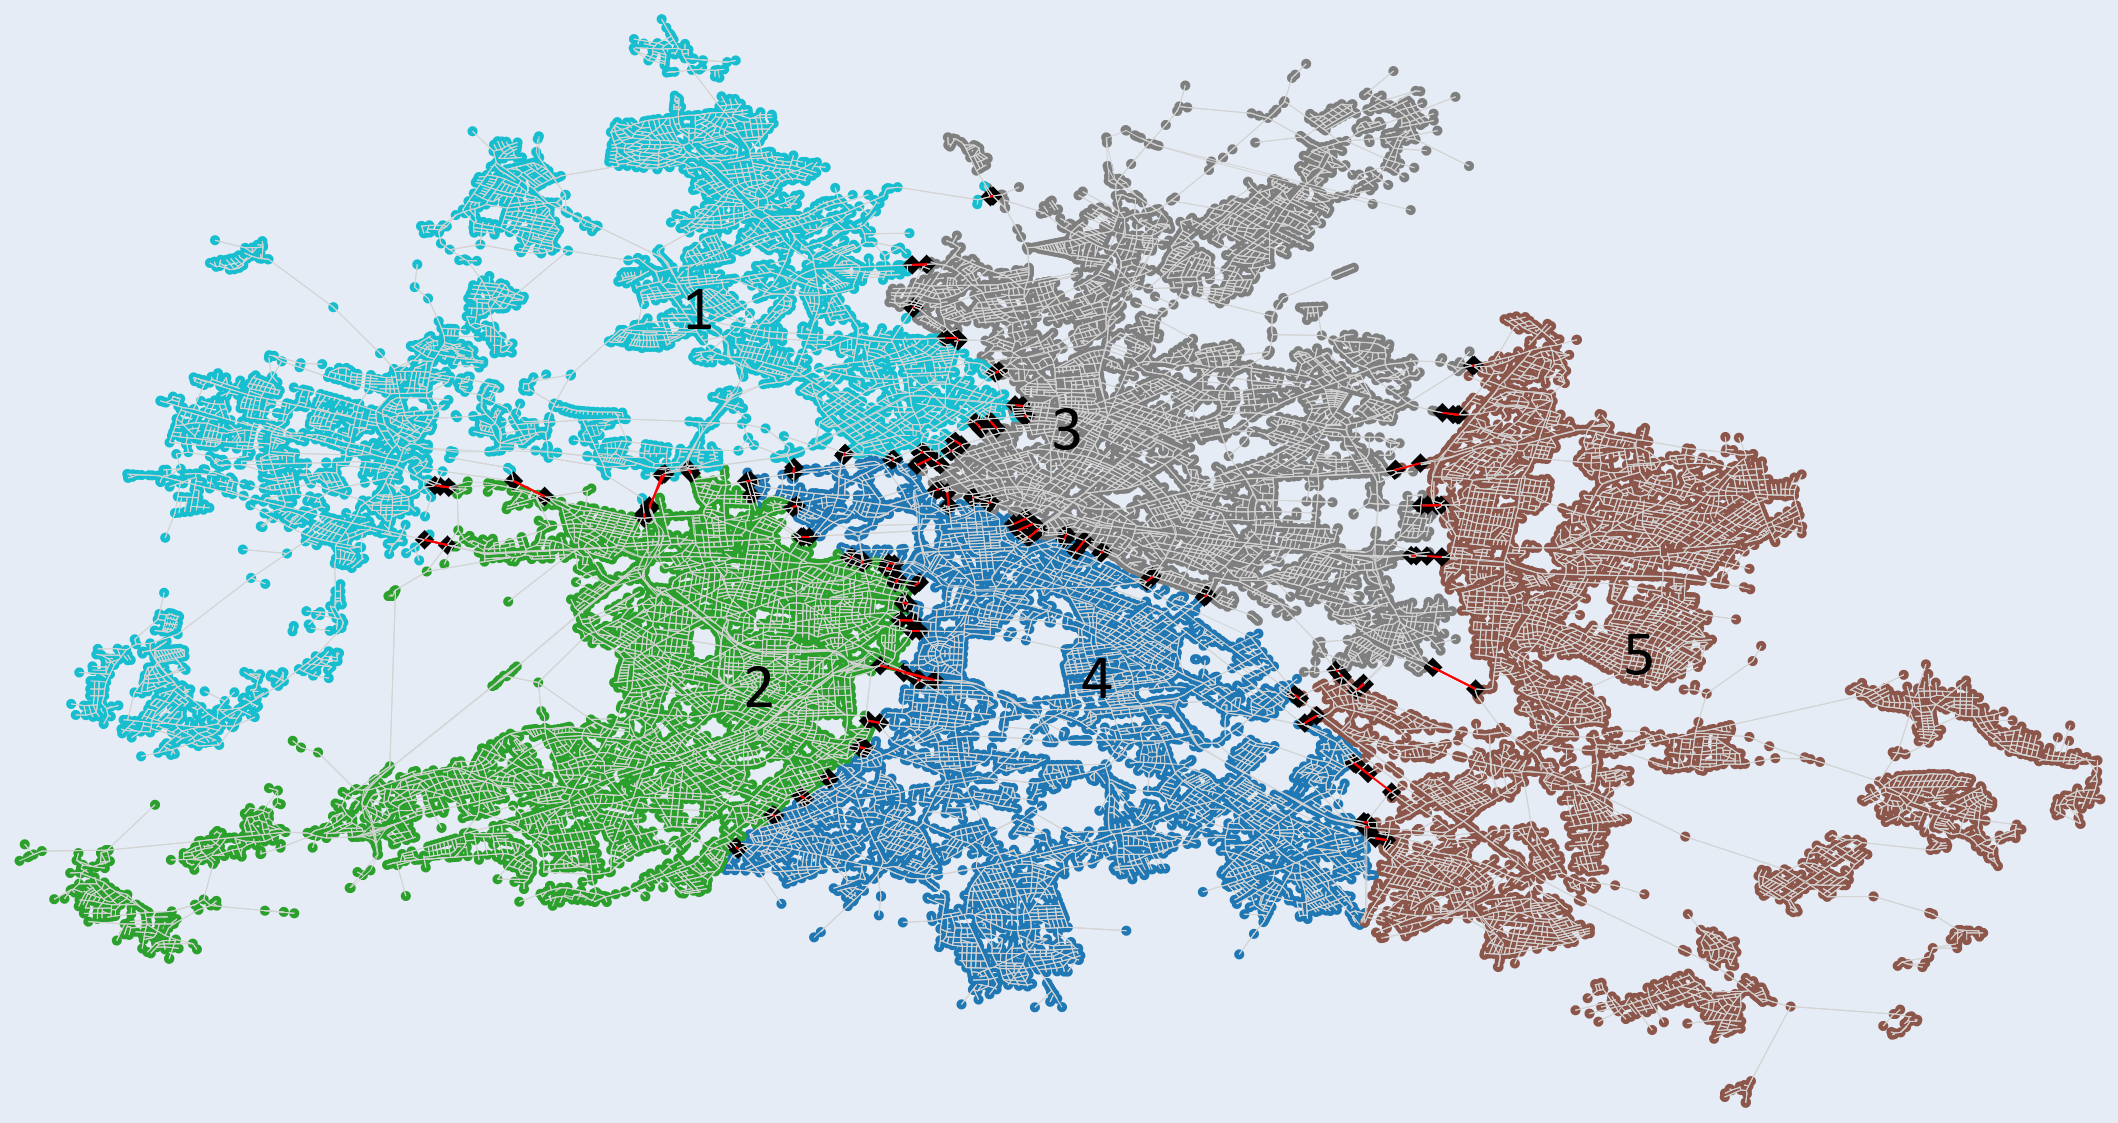
\includegraphics[width=0.95\linewidth,height=2.2in]{images/berlin_acas.png}
		\caption{ACA-separated Berlin road network. Numbers in black represent ACA ids}
		\label{fig:berlin_a}
	\end{subfigure}
	\begin{subfigure}{\linewidth}
		\centering
		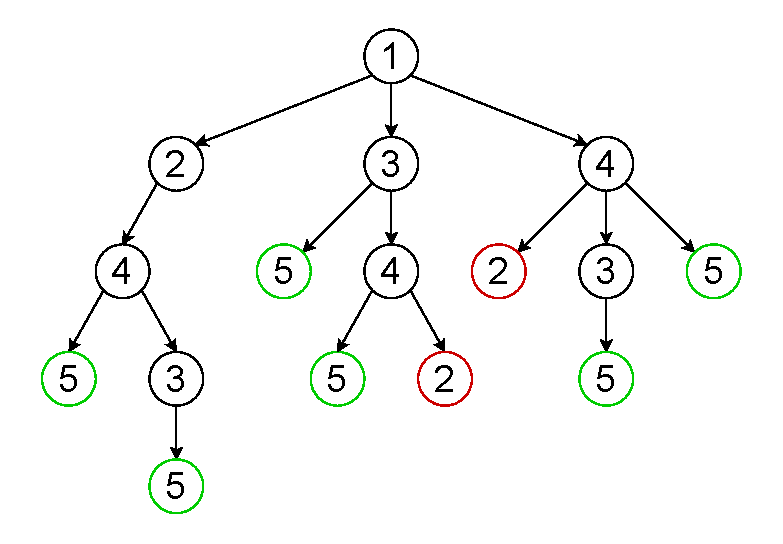
\includegraphics[width=0.95\linewidth,height=2.2in]{images/tree_search.pdf}
		\caption{Tree sequence of cooperative MCSPS between the ACAs for a route from area 1 to area 5}
		\label{fig:berlin_b}
	\end{subfigure}
	\caption{Example ACA system configuration and MCSPS exploration}
	\label{fig:berlin}
\end{figure}

As for the implementation, each ACA operates in two phases. During the first phase, the ACA attempts to route the vehicles starting in its own area of control. If the destination belongs to the same area, then the ACA computes and selects a complete multicriteria route for the vehicle. Otherwise, the ACA computes partial routes to the borders of its area and selects the next area to continue the routes in. The continuation request is sent to the neighboring ACA and a response expectation is logged.

The second phase of the method focuses on cooperative operation, where the ACA processes messages from its neighbors and communicates its state to the MA. This phase can be divided into three sub-phases which the algorithm iterates through until a termination signal is received. In the first phase, the agent processes all tasks in the internal queue. These tasks are route extension requests received from the neighbors and can either be completed in its area or extended to the area borders and sent further, depending on the arrival location. This sub-phase is largely similar in operation to phase one, with the main difference being that multicriteria queries start not from the departure position, but from incoming partial routes on a border of the area.

The second sub-phase is dedicated to receiving and processing incoming messages from other ACAs. In total, there are five types of messages passed between the agents. Message \textbf{\texttt{continueRoute}} is a request to a neighbor ACA to continue partially constructed routes in its area, containing the planning token and the open labels on the border. Type \textbf{\texttt{routeNotFound}} is used to notify the preceding ACA of a failure in route extension and return the token back. A message of type \textbf{\texttt{foundRoute}} is sent to the preceding agent with all labels corresponding to completed candidate routes and the planning token. \textbf{\texttt{acceptedRoute}} is a message sent by the origin ACA to the destination one to notify it of the chosen route to be reconstructed, and \textbf{\texttt{finishedRoute}} is a message sent to the previous ACA in the selected route to rebuild the route from its labels. This message contains the partially rebuilt route from the current border to the destination.

The third sub-phase ensures the ACAs successfully exit when all vehicles are routed. If an ACA has no tasks to perform and awaits no routes from the neighbors, it notifies the MA of its inactivity. If the MA receives inactivity notifications from all ACAs, it notifies all of them of successful completion, after which the ACAs can break the loop and return computed routes.

This algorithm is directly called by the ACAs when they receive proactive routing requests from the master agent (Algorithm \ref{alg:MA}, line 8). In case of reactive rerouting, several steps are performed prior to the planning procedure. First, each ACA checks if there are edges with expected traffic jams in its area. If these exist, the agent selects a portion of the vehicles that will traverse the edges in question in the upcoming interval. The current routes for these vehicles are removed from the predictions, and the vehicle set is passed as input to Algorithm \ref{alg:cooperative-routing-part1}.

The result of an MCSPS procedure is a Pareto set of candidate routes. Selecting a singular solution from the Pareto set is an important subproblem that can significantly affect system performance. To solve this task, we use the R-method \cite{R-method}. Using a combination of priority and criteria ranking, this method selects solutions based not only on user-defined priorities, but also on solution quality. Another advantage of the method is that, instead of requiring importance weights assigned to individual criteria, it works with priority ordering from the highest to the lowest one. This increases the ease of use for an average user, since it is much easier to select a criteria ordering than to quantize one's preferences.

\section{Simulations and Results}
\subsection{Experiment Setting}
An experimental analysis of the algorithm in this research is conducted using SUMO \cite{SUMO}, an open-source microscopic traffic simulator. Accumulation of traffic information and communication with vehicles is implemented using the traffic control interface TraCI \cite{traci}.

\begin{table}[t]
	\centering
		\begin{tabular}{lrrrr}
			\toprule
            parameter & \# junctions& \# roads& \# vehicles& road length (km)\\
            \midrule
            grid& 180& 610& 4000& 48.9\\
            InTAS& 3332& 7942& 28200 & 717.23\\
			\bottomrule
		\end{tabular}
    \caption{parameters of simulation scenarios}
	\label{tab:scenarios}
\end{table}

\begin{figure*}
	\centering
	\begin{subfigure}{0.49\linewidth}
		\centering
		
\includegraphics[height=2.5in]{images/grid.png}
		\caption{Grid}
		\label{fig:grid}
	\end{subfigure}
	\begin{subfigure}{0.49\linewidth}
		\centering
		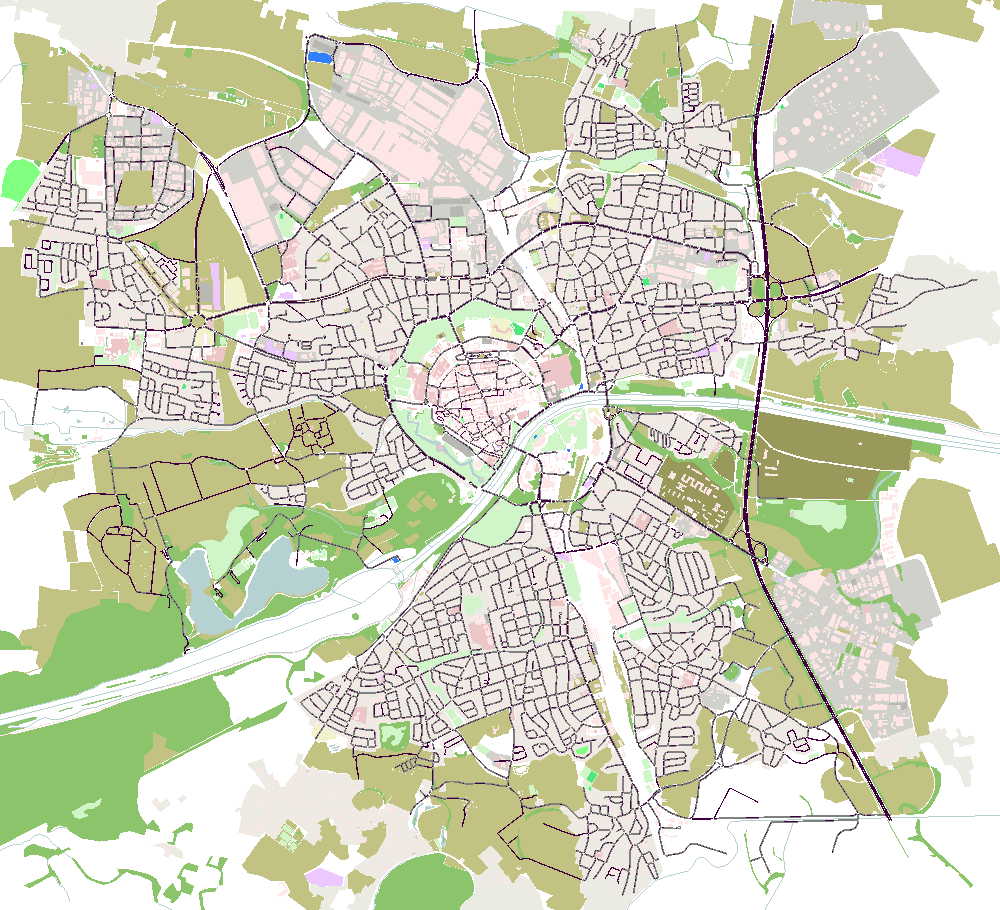
\includegraphics[height=2.5in, width=\linewidth]{images/intas.png}
		\caption{InTAS}
		\label{fig:intas}
	\end{subfigure}
	\caption{Testing scenarios in SUMO}
	\label{fig:scenarios}
\end{figure*}

The experiments were conducted on two scenarios, the main properties of which are presented in Figure \ref{fig:scenarios} and Table \ref{tab:scenarios}. The first scenario is based on a 10-by-15 grid network created using the NetGenerate tool provided in SUMO. There are horizontal fringe edges at all intersections from both sides, all roads in the network have two lanes and the speed limit of 13.9 m/s (50 km/h). Every junction is regulated by a standard-cycle traffic light. All traffic in this scenario arrives and departs at the fringes of the grid. The origin and destination edges of all vehicles are selected at random. The second scenario is the Ingolstadt Traffic Scenario (InTAS) \cite{InTAS}. This is a realistic simulation of Ingolstadt, with the traffic generated from activity patterns. We performed our experiments on four hours of simulation representing the morning peak hours from 7:00 to 11:00. The graphs were partitioned between the ACAs using the KaHIP framework \cite{kahip} to minimize the number of border edges. SUMO uses vehicle teleportation to prevent grid locks. In order to properly analyze traffic congestion in our simulations, we disabled teleportations due to traffic jams, leaving the ones caused by prolonged yield and wrong lane position enabled to prevent deadlocks. The MCSPS was augmented with $\epsilon$-pruning heuristic \cite{heur_t-kPC-MLS} with $\epsilon=0.99$. The rerouting interval $\Delta_r$ was set to 60 seconds, and the portion of rerouted vehicles to 0.85 for both algorithms. The synchronization interval $\Delta_s$ was set to 20 seconds. For all of the scenarios and configurations discussed below, the tests were repeated 10 times to account for the randomness in the simulations.

\subsection{Agent Number Analysis}
Due to only non-repeating agent sequences being allowed in cooperative route planning, some of more beneficial routes may be overlooked by the system. This is possible if the best route winds through the border between two ACAs multiple times. Generally speaking, this is a relatively rare occurrence that can happen if the area borders are set poorly. Nevertheless, we analyzed this effect by simulating the scenarios with different numbers of ACAs. The results of these simulations are in Table \ref{tab:agents}.

\begin{table*}
    \centering
    \begin{tabular}{crrrrrrrr}\toprule
         metrics& \multicolumn{4}{c}{grid} & \multicolumn{4}{c}{InTAS}\\\midrule
         & S & 1 & 2 & 3 & S & 1 & 2 & 3 \\
         distance, m& 923.71 &943.43 & 932.42&927.81 & 5012.36 & 4809.72 & 4921.35 & 4795.63\\
         time, s& 294.44 & 222.00 & 240.38& 232.88 & 927.59 & 657.07 & 660.92 & 627.82\\
         fuel, g& 182.26 & 158.10& 166.22& 162.14& 597.07 & 433.77 & 438.13 & 420.03\\
         \# teleportations& 65.00 & 0.00& 4.90 & 0.50 & 1183.00 & 154.00& 101.30& 58.40\\\bottomrule
    \end{tabular}
    \caption{Mean performance metrics depending on the agent number. "S" refers to standard scenario without optimization, numbers "1", "2", "3" represent the number of ACAs.}
    \label{tab:agents}
\end{table*}

\begin{table}
    \centering
    \begin{tabular}{ccc} \toprule
        \# agents & grid & InTAS\\\midrule
        1 & 0.006 & 4.250\\
        2 & 0.002 & 1.073\\
        3 & 0.001 & 0.308\\
        \bottomrule
    \end{tabular}
    \caption{Mean runtimes of MCSPS for singular ACAs}
    \label{tab:sps}
\end{table}

The metrics we analyzed are route distance, route time, fuel consumption, and number of teleportations in the simulation. The first conclusion to be drawn from the table is that for any number of agents, the system provides a significant positive effect on traffic in both scenarios. For the grid scenario, the distance improvement is negligible. This is explained by the fact that the system reroutes some of the vehicles via slightly longer routes to improve the dynamic metrics. This is evident from 20\% to 30\% improvements in time and fuel consumption virtually absent teleportations. The lack of improvement in traversed distance is logical for the grid network, since a vehicle can travel between any two points in a straightforward Manhattan distance which cannot be minimized further. In fact, the distance being increased by at most 2\% is a good indicator, since the system manages to significantly improve traffic throughput with minimal detours.

Since InTAS is an irregular network, the system manages to improve not only the dynamic criteria, but distance too. Both time and fuel consumption in InTAS are improved by 30\% on average, with teleportations reduced by approximately 90\%. As for the optimal number of agents, we can draw an interesting conclusion. A system consisting of 2 agents performs noticeably worse 1- and 3- agent systems. This confirms our remark about winding routes that cross the border between ACAs multiple times. A 2-agent system has one long border between the agents, which makes it the most prohibitive in terms of multiple border crossings. While a higher number of agents increases the total border length, the borders become distributed between more ACA pairs, which means that the same route will likely cross borders between multiple agent pairs, not just one. Thus, a higher number of agents appears to be beneficial for system performance.

\subsection{MCSPS Analysis}
As stated earlier, multicriteria shortest path search is an NP-hard problem, which often limits its practical applicability. In this aspect, our system has two important advantages. Firstly, it can operate with any shortest path search algorithm, including more advanced and even metaheuristic ones. Secondly, its multiagent architecture parallelizes shortest path search in a certain manner. When an ACA sends a route continuation request to another agent, it works on another query instead of waiting idly for a response. Table \ref{tab:sps} gives average MCSPS runtimes for both scenarios and 4 planning criteria: distance, time, fuel, and edge number.

An ACA shortest path search query for a vehicle consists in expanding it through its own area only, either from the start position of a vehicle or from the border of the area. The average query runtime decreases significantly with the higher number of agents, which proves the parallelization abilities of the system. Naturally, a cooperative shortest path search involves more than one ACA. Let us consider 3 agents (e.g. 1, 2, 3) splitting the city evenly, and route query from area 1 to area 3. This involves two possible sequences: 1, 3 and 1, 2, 3. Agent 1 will not have to recompute routes to their borders, so we get 4 area-specific queries in total. For InTAS, this gives us 1.232 seconds as opposed to 4.250, which is a speedup of over 3 times. Thus, the cooperative multiagent approach not only enables parallel route computation, but also improves absolute MCSPS runtimes. As a result, the proposed system enables wider practical application of MCSPS and usage of its intrinsic advantages.

\subsection{Comparison with State-of-the-Art}
We compare our system to a recent state-of-the-art approach proposed by Ho et al. \cite{reference}. The reference algorithm, as we will call it here, has a similar approach to periodic reactive rerouting. However, it has a number of important distinctions. First of all, it uses the $k$-shortest path search approach \cite{kSP}. Second, it does not make use of parallelization, which hinders its scalability. Third, it is a purely rerouting method, with no proactive functionality. We consider this an overlook, since the approach still requires identical connection abilities to our system. For fairness, we set the two compared methods to use identical prediction models and parameters. The comparison was done with 3 ACAs. The reference algorithm used predicted time as its planning criterion. The results of this comparison are in Table \ref{tab:comparison}.

\begin{table*}
    \centering
    \begin{tabular}{crrrrrr}
    \toprule
        metric & \multicolumn{3}{c}{grid} & \multicolumn{3}{c}{InTAS}\\
        \midrule
         & S & R & 3 & S & R & 3 \\
         distance, m& 923.71 & 948.87 & 927.81 & 5012.36& 5031.64& 4795.63\\
         time, s& 294.44 & 224.80 & 232.88 & 927.59& 865.87& 627.82\\
         fuel, g& 182.26 & 153.41 & 162.14 & 597.07& 567.18& 420.03\\
         \# teleportations& 65.00 & 4.50 & 0.50 & 1183.00 & 934.90 & 58.40 \\
         \# reroutes& 0 & 641.40 & 0 & 0 & 957.90 & 0\\
         \bottomrule
    \end{tabular}
    \caption{Comparison of reference and multiagent rerouting approaches. "S" column refers to the standard scenario without optimization, "R" column is the performance of the reference algorithm, and "3" column is the result of the proposed multiagent system with 3 ACAs.}
    \label{tab:comparison}
\end{table*}

As can be seen, both systems achieve a varying degree of success in traffic optimization. In the grid scenario, the reference system does provide slightly better dynamic metrics, but loses in terms of distance. This is due to the fact that single-criterion shortest path search is focused solely on time optimization, while MCSPS considers several metrics at once and attempts to find a balance between them. For the larger and more complex InTAS, however, the multiagent system achieves significantly better performance across all metrics, improving the dynamic criteria by $25\%$. Of special interest is the total absence of reactive reroutes in the multiagent simulations. Therefore, the achieved result can be attributed to solely proactive routing. From a developer point of view, this presents proactive rerouting as a powerful approach that is unjustly overlooked. For the user, on the other hand, this may provide a better experience, since being rerouted mid-trip can be unpleasant and creates a negative impression of the system's reliability.

\section{Conclusion}
The proposed multi-agent system for dynamic rerouting offers several advantages over existing approaches. It outperforms centralized alternatives in scalability and robustness, which are critical in practice: computational capacity of existing ACAs can be increased to handle higher traffic intensity, while new agents can be seamlessly added to accommodate city growth, and full decentralization eliminates a single point of failure. It also leverages and extends multicriteria shortest path search, as MCSPS can be readily augmented with more elaborate, user-tailored criteria, including green-city metrics. Finally, ACA functionality can be expanded to other optimization domains such as traffic light control, public transport optimization, and car- and ride-sharing management.

We outline several immediate directions for future research. First, the optimal number and placement of ACAs could be studied in more detail, though this strongly depends on city geography. Second, a real-world deployment would involve only partial participation of traffic users, an aspect beyond the scope of this work. While the proposed system achieved its performance using solely proactive routing—suggesting capacity to compensate for incomplete penetration—traffic density prediction becomes more critical under partial observability. This may be addressed through historically informed approaches or more advanced predictive models, but remains a complex standalone problem requiring dedicated study.

%%%%%%%%%%%%%%%%%%%%%%%%%%%%%%%%%%%%%%%%%%%%%%%%%%%%%%%%%%%%%%%%%%%%%%%%

%%% The acknowledgments section is defined using the "acks" environment
%%% (rather than an unnumbered section). The use of this environment 
%%% ensures the proper identification of the section in the article 
%%% metadata as well as the consistent spelling of the heading.

\begin{acks}
\texttt{This work was supported by the Technology Agency of the Czech Republic, grant Bozek Vehicle Engineering National Center of Competence (TN02000054).}
\end{acks}

%%%%%%%%%%%%%%%%%%%%%%%%%%%%%%%%%%%%%%%%%%%%%%%%%%%%%%%%%%%%%%%%%%%%%%%%

%%% The next two lines define, first, the bibliography style to be 
%%% applied, and, second, the bibliography file to be used.

\bibliographystyle{ACM-Reference-Format} 
\balance
\bibliography{bibliography}

%%%%%%%%%%%%%%%%%%%%%%%%%%%%%%%%%%%%%%%%%%%%%%%%%%%%%%%%%%%%%%%%%%%%%%%%

\end{document}

%%%%%%%%%%%%%%%%%%%%%%%%%%%%%%%%%%%%%%%%%%%%%%%%%%%%%%%%%%%%%%%%%%%%%%%%

